% Figure 1 — the decision cascade of the deployment-decay instrument (PAPER_DRAFT_V4 §3).
% Standalone: compile with `pdflatex fig1_cascade.tex` (TikZ only, no extra packages).
% NOTE: written on a machine without LaTeX — compile-test before submission.
% Layout mirrors the mermaid draft in PAPER_DRAFT_V4.md §3; colors: concept/verified-null
% green, noise-confounded amber, vacuous red, abstain grey.
\documentclass[tikz,border=6pt]{standalone}
\usetikzlibrary{shapes.geometric,arrows.meta,positioning,fit}
\begin{document}
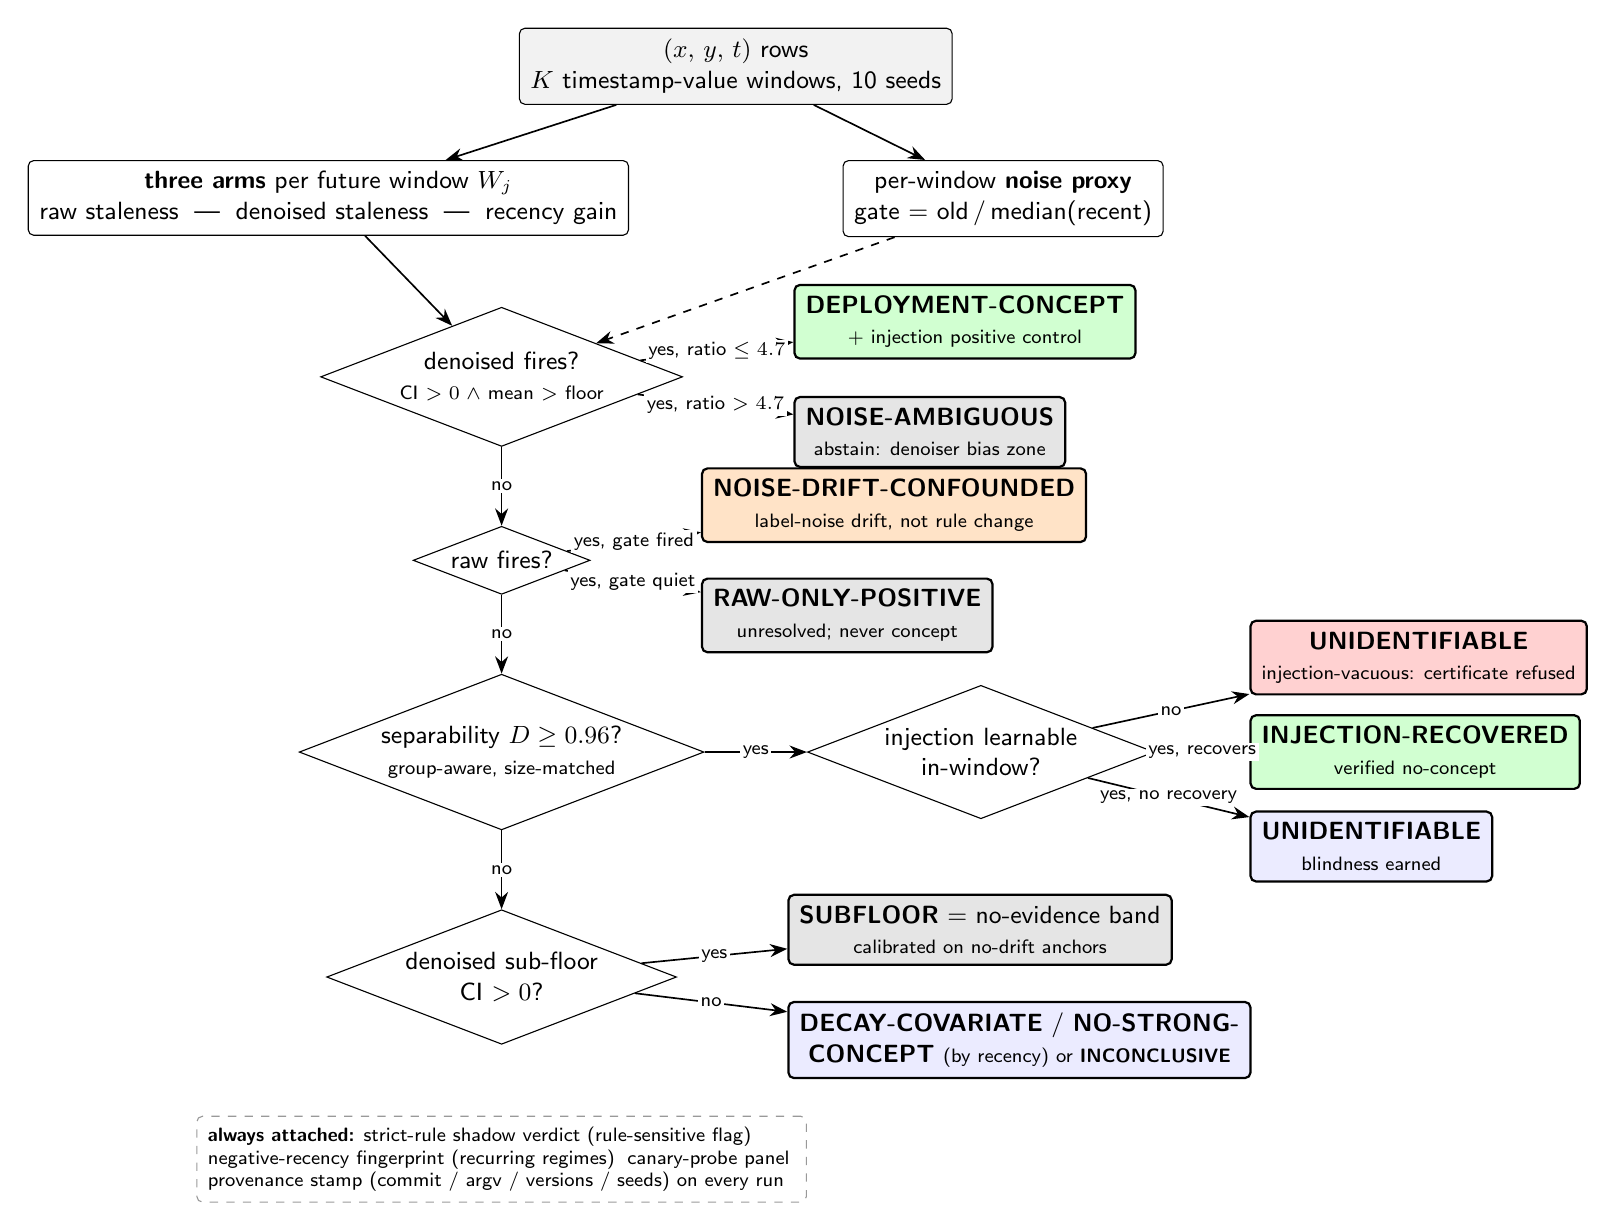
\begin{tikzpicture}[
  font=\small\sffamily,
  node distance=5mm and 7mm,
  box/.style={draw,rounded corners=2pt,align=center,inner sep=4pt,minimum height=8mm},
  dec/.style={draw,diamond,aspect=2.6,align=center,inner sep=1.5pt},
  verd/.style={box,thick},
  good/.style={verd,fill=green!18},
  warn/.style={verd,fill=orange!22},
  bad/.style={verd,fill=red!18},
  grey/.style={verd,fill=black!10},
  neut/.style={verd,fill=blue!8},
  lab/.style={font=\scriptsize\sffamily,midway,fill=white,inner sep=1pt},
  arr/.style={-{Stealth[length=2.2mm]},semithick}
]

% ---------- inputs ----------
\node[box,fill=black!5] (data) {$(x,\,y,\,t)$ rows\\ $K$ timestamp-value windows, 10 seeds};
\node[box,below left=7mm and -14mm of data] (arms)
  {\textbf{three arms} per future window $W_j$\\ raw staleness\; |\; denoised staleness\; |\; recency gain};
\node[box,below right=7mm and -14mm of data] (gate)
  {per-window \textbf{noise proxy}\\ gate $=$ old\,/\,median(recent)};
\draw[arr] (data) -- (arms);
\draw[arr] (data) -- (gate);

% ---------- cascade ----------
\node[dec,below=9mm of arms,xshift=22mm] (d1) {denoised fires?\\ \scriptsize CI $>0\;\wedge$ mean $>$ floor};
\draw[arr] (arms) -- (d1);
\draw[arr,dashed] (gate) -- (d1);

\node[good,right=14mm of d1,yshift=7mm] (concept) {\textbf{DEPLOYMENT-CONCEPT}\\ \scriptsize + injection positive control};
\node[grey,right=14mm of d1,yshift=-7mm] (ambig) {\textbf{NOISE-AMBIGUOUS}\\ \scriptsize abstain: denoiser bias zone};
\draw[arr] (d1) -- node[lab]{yes, ratio $\le 4.7$} (concept);
\draw[arr] (d1) -- node[lab]{yes, ratio $> 4.7$} (ambig);

\node[dec,below=10mm of d1] (d2) {raw fires?};
\draw[arr] (d1) -- node[lab]{no} (d2);
\node[warn,right=14mm of d2,yshift=7mm] (noise) {\textbf{NOISE-DRIFT-CONFOUNDED}\\ \scriptsize label-noise drift, not rule change};
\node[grey,right=14mm of d2,yshift=-7mm] (rawonly) {\textbf{RAW-ONLY-POSITIVE}\\ \scriptsize unresolved; never concept};
\draw[arr] (d2) -- node[lab]{yes, gate fired} (noise);
\draw[arr] (d2) -- node[lab]{yes, gate quiet} (rawonly);

\node[dec,below=10mm of d2] (d3) {separability $D \ge 0.96$?\\ \scriptsize group-aware, size-matched};
\draw[arr] (d2) -- node[lab]{no} (d3);

\node[dec,right=13mm of d3] (d4) {injection learnable\\ in-window?};
\draw[arr] (d3) -- node[lab]{yes} (d4);
\node[bad,right=12mm of d4,yshift=12mm] (vac) {\textbf{UNIDENTIFIABLE}\\ \scriptsize injection-vacuous: certificate refused};
\node[good,right=12mm of d4] (recov) {\textbf{INJECTION-RECOVERED}\\ \scriptsize verified no-concept};
\node[neut,right=12mm of d4,yshift=-12mm] (earned) {\textbf{UNIDENTIFIABLE}\\ \scriptsize blindness earned};
\draw[arr] (d4) -- node[lab]{no} (vac);
\draw[arr] (d4) -- node[lab]{yes, recovers} (recov);
\draw[arr] (d4) -- node[lab]{yes, no recovery} (earned);

\node[dec,below=10mm of d3] (d5) {denoised sub-floor\\ CI $> 0$?};
\draw[arr] (d3) -- node[lab]{no} (d5);
\node[grey,right=14mm of d5,yshift=6mm] (subfloor) {\textbf{SUBFLOOR} $=$ no-evidence band\\ \scriptsize calibrated on no-drift anchors};
\node[neut,right=14mm of d5,yshift=-8mm] (nulls) {\textbf{DECAY-COVARIATE} / \textbf{NO-STRONG-}\\ \textbf{CONCEPT} \scriptsize(by recency) or \textbf{INCONCLUSIVE}};
\draw[arr] (d5) -- node[lab]{yes} (subfloor);
\draw[arr] (d5) -- node[lab]{no} (nulls);

% ---------- side-channel annotations ----------
\node[box,draw=black!40,dashed,below=9mm of d5,align=left,font=\scriptsize\sffamily] (side)
  {\textbf{always attached:} strict-rule shadow verdict (rule-sensitive flag)\; \\
   negative-recency fingerprint (recurring regimes)\; canary-probe panel\; \\
   provenance stamp (commit / argv / versions / seeds) on every run};

\end{tikzpicture}
\end{document}
